\documentclass{jhwhw}
\author{Ian Malerich}
\title{Math 481: Homework 1}
\usepackage{amssymb}
\usepackage{mathtools}
\usepackage{graphicx}
\usepackage{breqn}

\graphicspath{ {png/} }

\usepackage{minted}
\usepackage{xcolor}
\usemintedstyle{friendly}
\definecolor{llgray}{gray}{0.9}

\begin{document}

\problem{}

\indent{
    Use Matlab (or some other program) to calculate the polynomial which interpolates the function
    \begin{gather}
	    f(x) = \frac{1}{1 + 25x^2}
    \end{gather}
    at equally spaced points between -1 and 1, in steps of 0.25. You can use Matlab built-in 
    to find the polynomial. \\
}

\indent{
    Plot the original function (in default color blue) and the interpolating polynomial
    (in red), and put circles around the interpolation points. Make sure you use enough points
    so that you get a smooth-looking curve.
}

\solution

    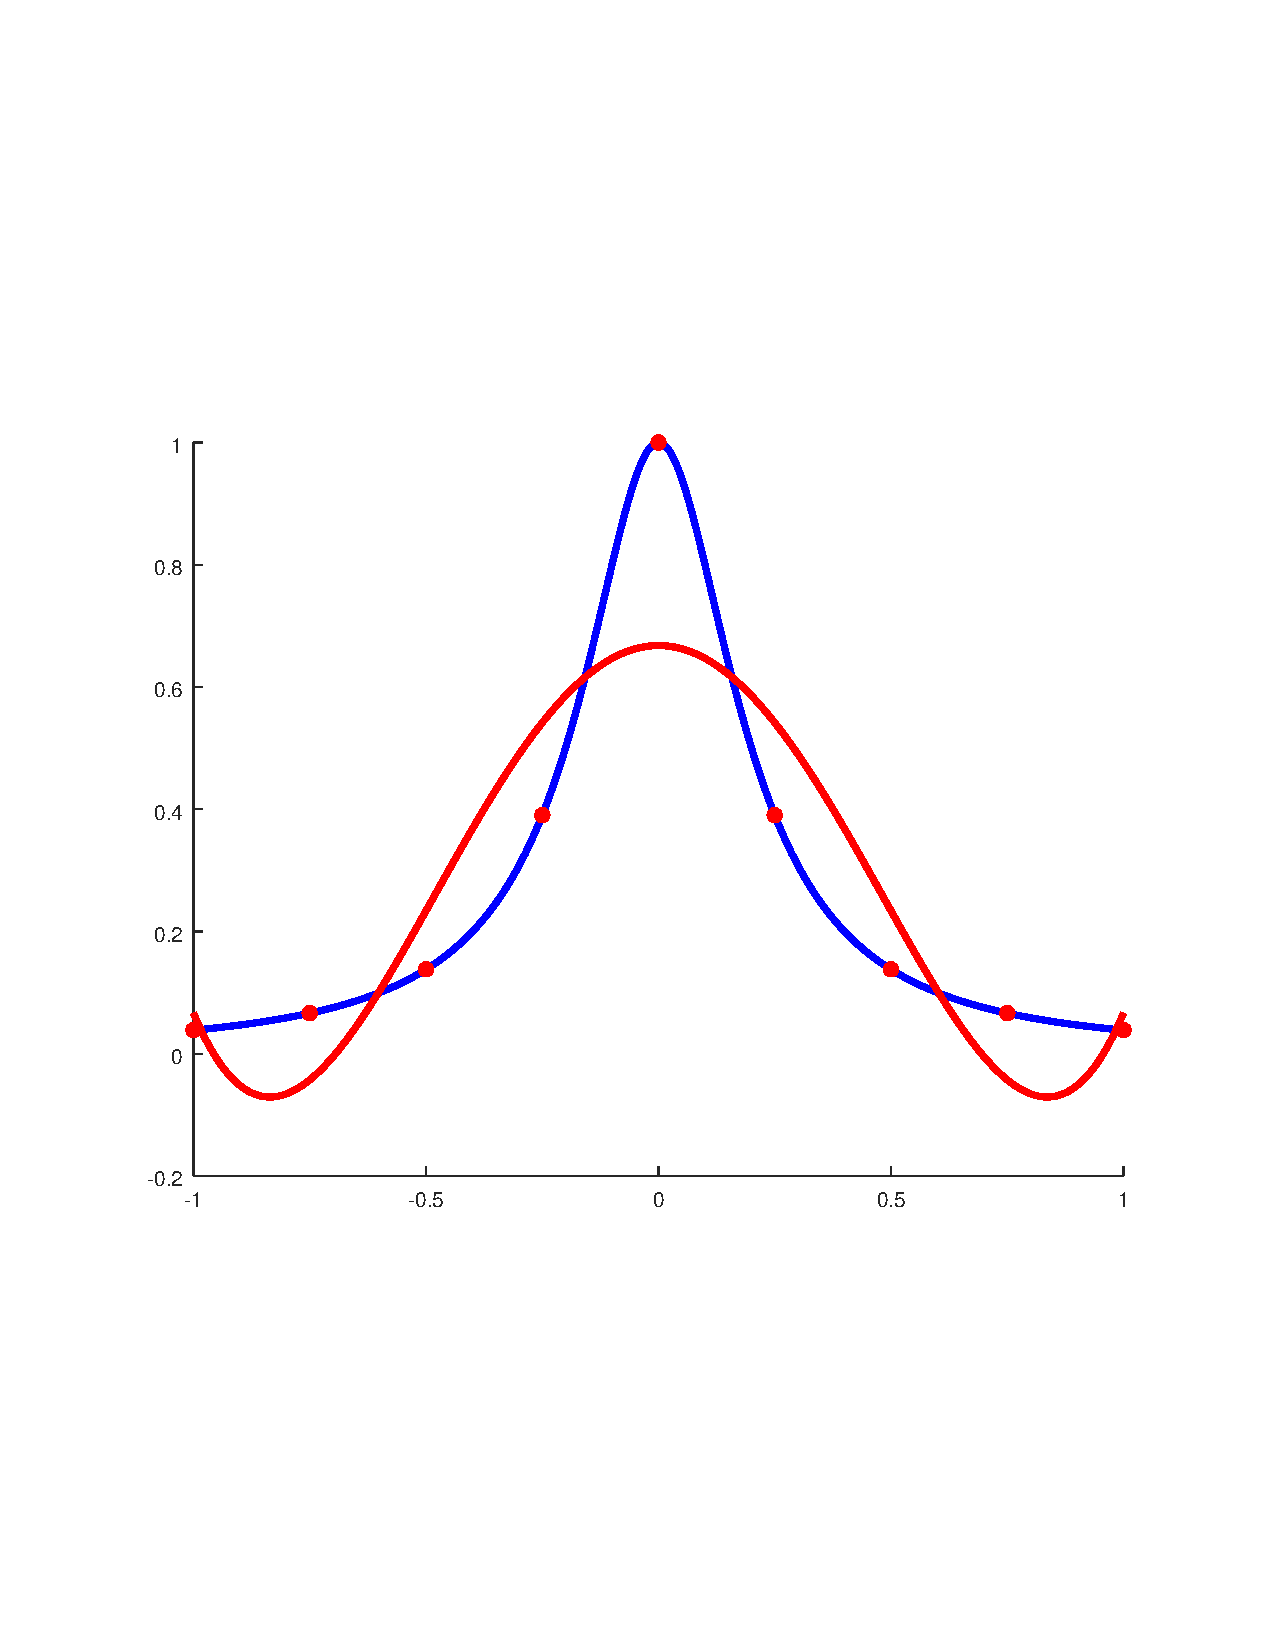
\includegraphics[scale=0.75]{p1}
    {\centering
	    \inputminted[linenos,bgcolor=llgray,frame=lines,framesep=2mm]{octave}{p1.m}}

\problem{}

\begin{enumerate}
    \item Given a point $x_0$ and a step size h, use Lagrange polynomials to find the quadratic polynomial
	    which interpolates a function f(x) at the points $x_0$-2h, $x_0$, and $x_0$+h.
    \item Integrate the polynomial on [$x_0$-2h, $x_0$+h] to produce an integration formula.
	    Use the formula to estimate $\int_{0}^{3} e^{-x} dx$.
\end{enumerate}

\solution

    \part
    Denote the Lagrange polynomial P(t) given by \\
    \begin{dmath*}
	P(t) = 
	    f(x_0 - 2h)\frac{(t-t_1)(t-t_2)}{(t_0-t_1)(t_0-t_2)} \\
	    + f(x_0)\frac{(t-t_0)(t-t_2)}{(t_1-t_0)(t_1-t_2)} \\
	    + f(x_0 + h)\frac{(t-t_0)(t-t_1)}{(t_2-t_0)(t_2-t_1)} \\
    \end{dmath*}
    \bigbreak
    In this case we have $t_0 = x_0 - 2h$, $t_1 = x_0$, and $t_2 = x_0 + h$. \\
    Next we make the necessary substitutions and simplify the different parts of P(t). \\
    \begin{flalign*}
	(t - t_1)(t - t_) &= (t - x_0)(t - (x_0 + h)) &\\
	(t - t_0)(t - t_2) &= (t - x_0 + 2h)(t - x_0 - h) &\\
	(t - t_0)(t - t_1) &= (t - x_0 + 2h)(t - x0) &\\
	(t_0-t_1)(t_0-t_2) &= ((x_0-2h) - x_0)((x_0-2h) - (x_0 + h)) &\\
	&= (-2h)(x_0 - 2h - x_0 - h) &\\
	&= (-2h)(-3h) &\\
	&= 6h^2 &\\
	&= (t - x_0)(t - x_0 - h) &\\
	(t_1-t_0)(t_1-t_2) &= (x_0 - (x_0 - 2h))(x_0 - (x_0 + h)) &\\
	&= (2h)(-h) &\\
	&= -2h^2 &\\
	(t_2 - t_0)(t_2-t_1) &= ((x_0 + h)-(x_0 - 2h))((x_0 - 2h) - x0) &\\
	&= (3h)(h) &\\
	&= 3h^2 &\\
    \end{flalign*}

    Thus we arrive at the following equation
    \begin{dmath*}
	P(t) = 
	    \frac{f(x_0 - 2h)}{6h^2}(t - x_0)(t - x_0 - h) \\
	    + \frac{f(x_0)}{-2h^2}(t - x_0 + 2h)(t - x_0 - h) \\
	    + \frac{f(x_0 + h)}{3h^2}(t - x_0 + 2h)(t - x_0) \\
    \end{dmath*}

    \bigbreak
    In the GNU Octave code below, P(t) is broken up into parts
    L0, L1, L2 which are defined on lines 26-28 of the code.
    The graph below shows an example case of the quadratic Lagrange polynomial for the function 
    $e^{-x}$ with $x_0 = 2$, $h = 1$. The original function is drawn in blue, while the Lagrange polynomial
    drawn is in red. \\

    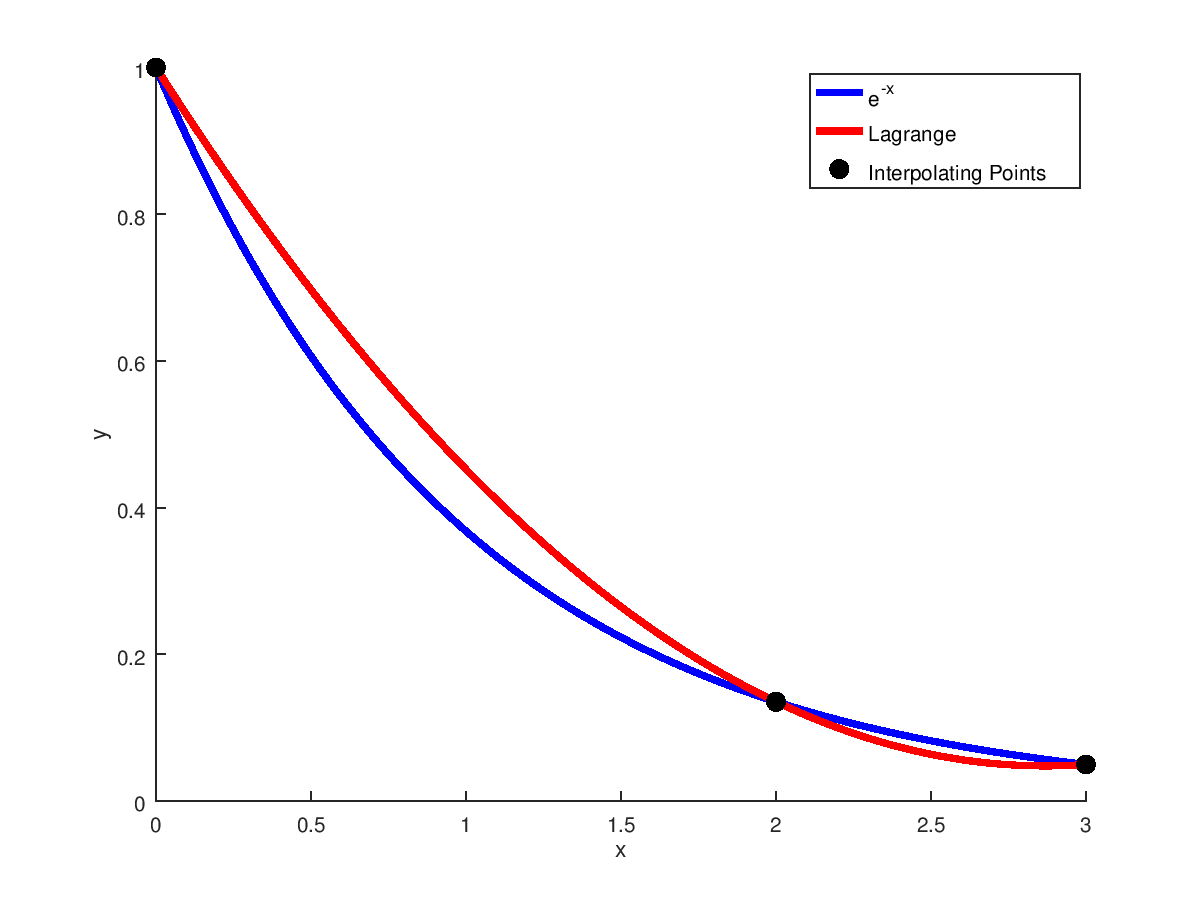
\includegraphics[scale=0.75]{p2}
    \part
    In order to integrate P(t), first expand each term to produce

    \begin{dmath*}
	P(t) = 
	    \frac{f(x_0 - 2h)}{6h^2}(-ht + hx_0 + t^2 + x_0^2) \\
	    + \frac{f(x_0)}{-2h^2}(-2h^2 + ht - hx_0 + t^2 - 2tx_0 + x_0^2) \\
	    + \frac{f(x_0 + h)}{3h^2}(2ht - 2hx_0 + t^2 - 2tx_0 + x_0^2) \\
    \end{dmath*}

    Integrating both sides produces

    \begin{dmath*}
	\int_{x_0-2h}^{x_0+h}P(\tau )d\tau = 
	    \frac{f(x_0 - 2h)}{6h^2}\int_{x_0-2h}^{x_0+h}(-ht + hx_0 + t^2 + x_0^2) d\tau \\
	    + \frac{f(x_0)}{-2h^2}\int_{x_0-2h}^{x_0+h}(-2h^2 + ht - hx_0 + t^2 - 2tx_0 + x_0^2) d\tau \\
	    + \frac{f(x_0 + h)}{3h^2}\int_{x_0-2h}^{x_0+h}(2ht - 2hx_0 + t^2 - 2tx_0 + x_0^2) d\tau \\
    \end{dmath*}

    \begin{dmath*}
	\int_{x_0-2h}^{x_0+h}P(\tau )d\tau = 
	    \frac{f(x_0 - 2h)}{6h^2} 
		(-\frac{h}{2}\tau^2 + hx_0\tau + \frac{1}{3}\tau^3 - x_0\tau^2 + x_0^2\tau) 
		\rvert_{x_0-2h}^{x_0+h} \\
	    + \frac{f(x_0)}{-2h^2} 
		(-2h^2\tau + \frac{h}{2}\tau^2 - hx_0\tau + \frac{1}{3}\tau^3 - x_0\tau^2 + x_0^2\tau) 
		\rvert_{x_0-2h}^{x_0+h} \\
	    + \frac{f(x_0 + h)}{3h^2} 
		$(h\tau^2 - 2hx_0\tau + \frac{1}{3}\tau^3 - x_0\tau^2 + x_0^2\tau)$\rvert_{x_0-2h}^{x_0+h} \\
    \end{dmath*}

    Each indefinite is given by intL0, intL1, $\&$ intL2 in the Octave code below. Each integral on
    $[x_0 - 2h, x_0 + h]$ is evaluated at lines 44-46 and assigned to evalL0, evalL1, $\&$ evalL2.
    These are then multiplied by their corresponding constants producing k0, k1, and k2 which are then summed
    to produce the result of the integral of P(t) on the given bounds.
    Line 54 of the Octave code produces the actual integral of f using one of Octaves built in numerical 
    integration methods.
    Line 55 of the Octave code produces the estimate of the integral of f, computed by evaluating the
    integral of P(t).

    \begin{align*}
	\int_{0}^{3}e^{-x}dx &= 0.95021 &\\
	\int_{0}^{3}P(t)dt &= 1.0545 &\\
    \end{align*}

    \raggedright
    The estimate of the integral via the Lagrange polynomial has an error of 0.10429.

    {\centering \inputminted[linenos,breaklines,bgcolor=llgray,frame=lines,framesep=2mm]{octave}{p2.m}}

\problem{}

    For k=2, Iserles calls these the Nystrom and Milne methods. That is, start with
    \begin{gather}
	    y(t_{n+2}) = y(t_n) + \int_{t_n}^{t_{n+2}}f(\tau , y(\tau )) d\tau ,
    \end{gather}
    and interpolating at $t_n$, $t_{n+1}$ (explicit) or $t_n$, $t_{n+1}$, $t_{n+2}$ (implicit). \\
    Find the leading error term, and the order of the method, for both cases.

\solution

\problem{}

The IVP \\
\begin{gather}
    y' = -y + e^{-t}$cos(2t)$\\
    y(0) = 0
\end{gather}

has the true solution y(t) = $e^{-t}$sin(2t).
\indent{
    Solve it numerically, using Euler's method with 20, 40, 80, 160 steps from 0 to 1, and compute
    the global error at the endpoint for each stepsize. Verify that the error goes down approximately linearly.
}

\solution

    {\centering
	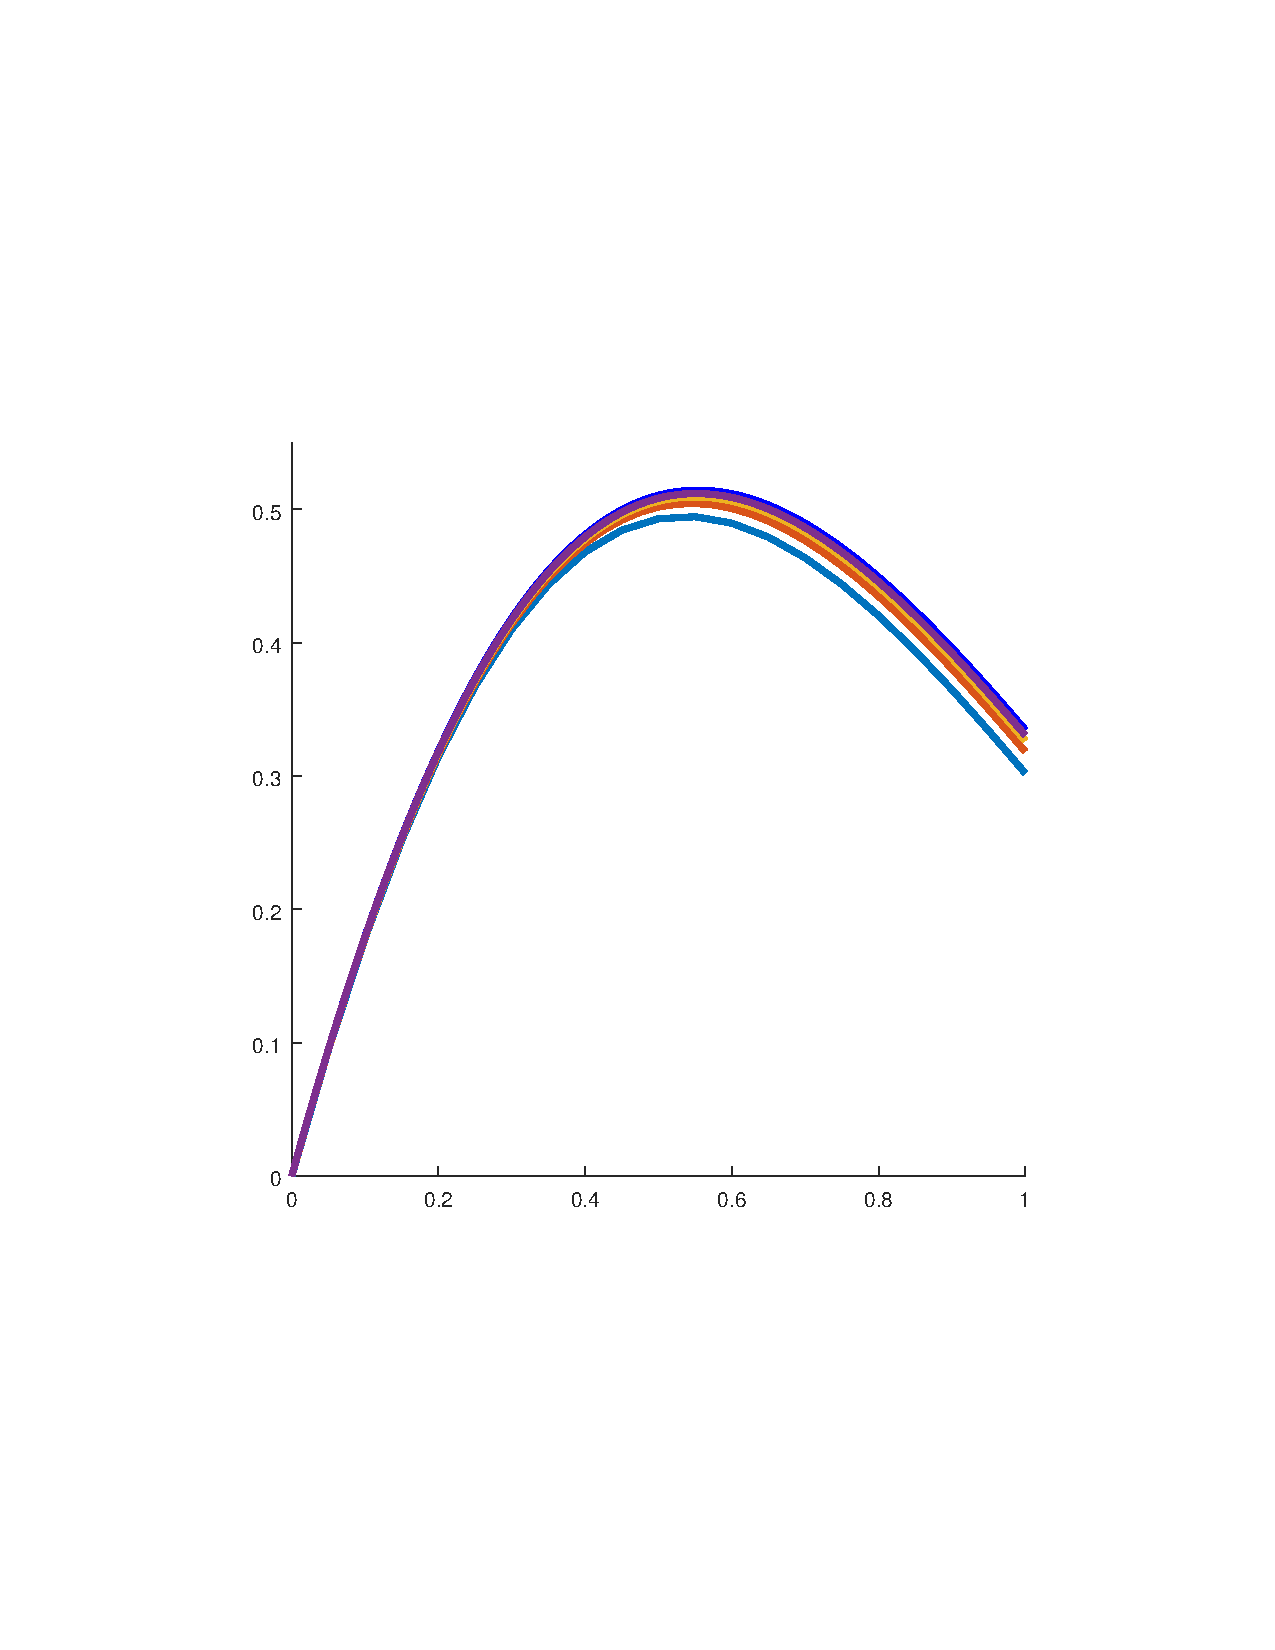
\includegraphics[scale=0.75]{p4} \\
	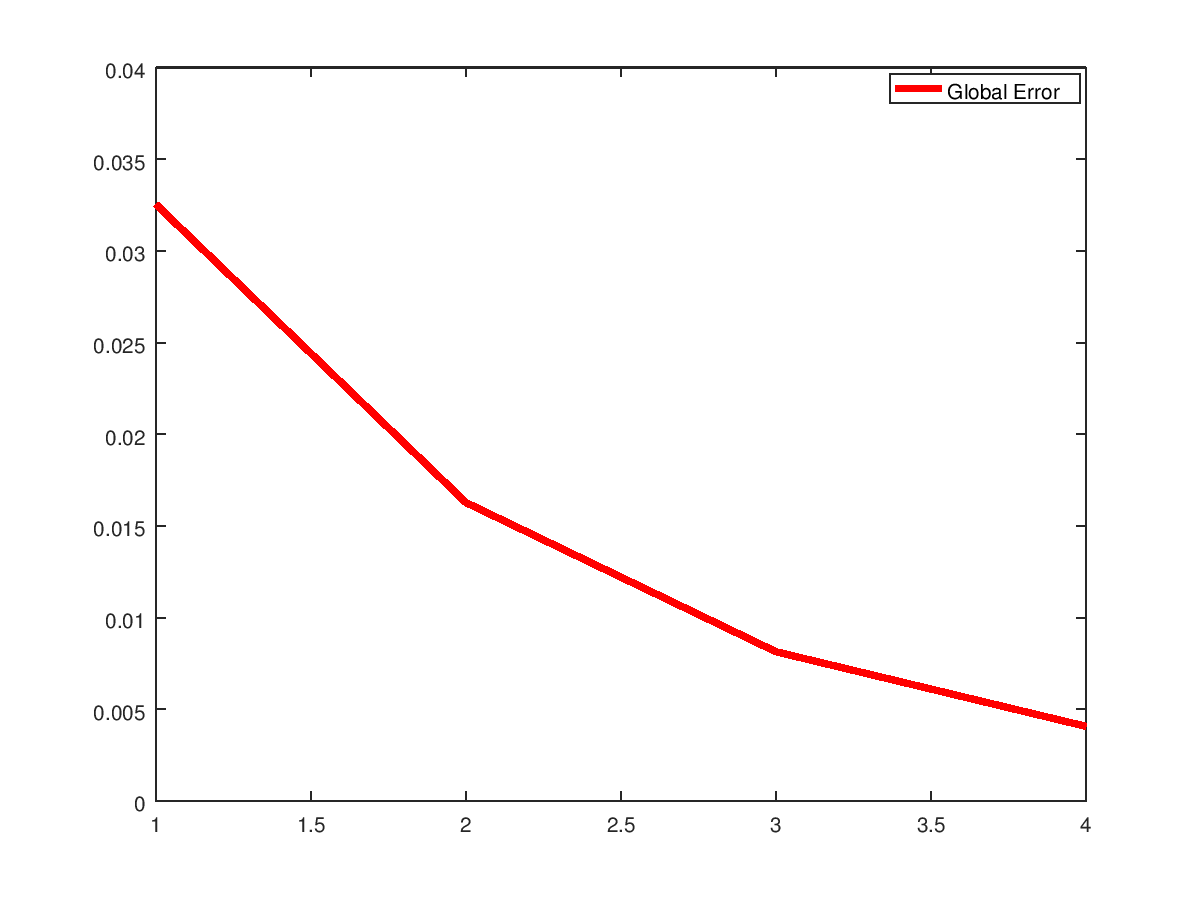
\includegraphics[scale=0.75]{p4_err} \\
    }
    \setlength\parindent{0pt}
    Note that the error term (graphed above) descends approximately linearly with respect to the step size.
    \inputminted[linenos,bgcolor=llgray,frame=lines,framesep=2mm]{octave}{p4.m}

\problem{}

Solve

\raggedright
\setlength\parindent{24pt}
    y''(t) = \begin{bmatrix}0 \\ -10\end{bmatrix} - 0.1y'(t), \\
    \bigbreak
    y(0) = \begin{bmatrix}0 \\ 0\end{bmatrix}$,$ \\
    \bigbreak
    y'(0) = \begin{bmatrix}10 \\ 10\end{bmatrix}
    \bigbreak

\setlength\parindent{0pt}
by using Euler's method with stepsize h = 0.1, until $y_2$ becomes 0 or negative. \\
Plot $y_1$ and $y_)$ as functions of t (horizontal and vertical distance as functions of time), and also
plot $y_2$ versus $y_1$. That will show the path of the object. It should look a bit like a parabola, but compressed
on the right because of friction.

\solution

    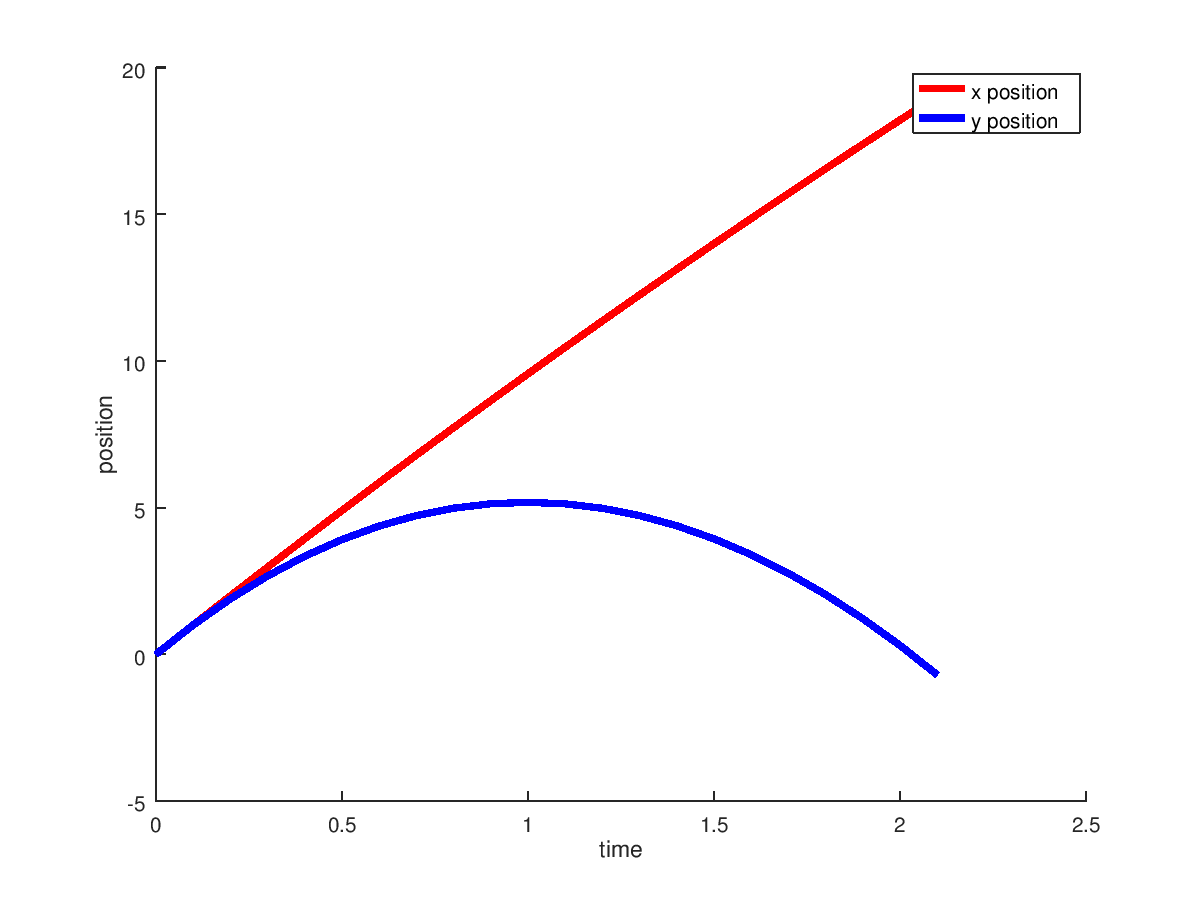
\includegraphics[scale=0.75]{p5_y1_y2_vs_time}
    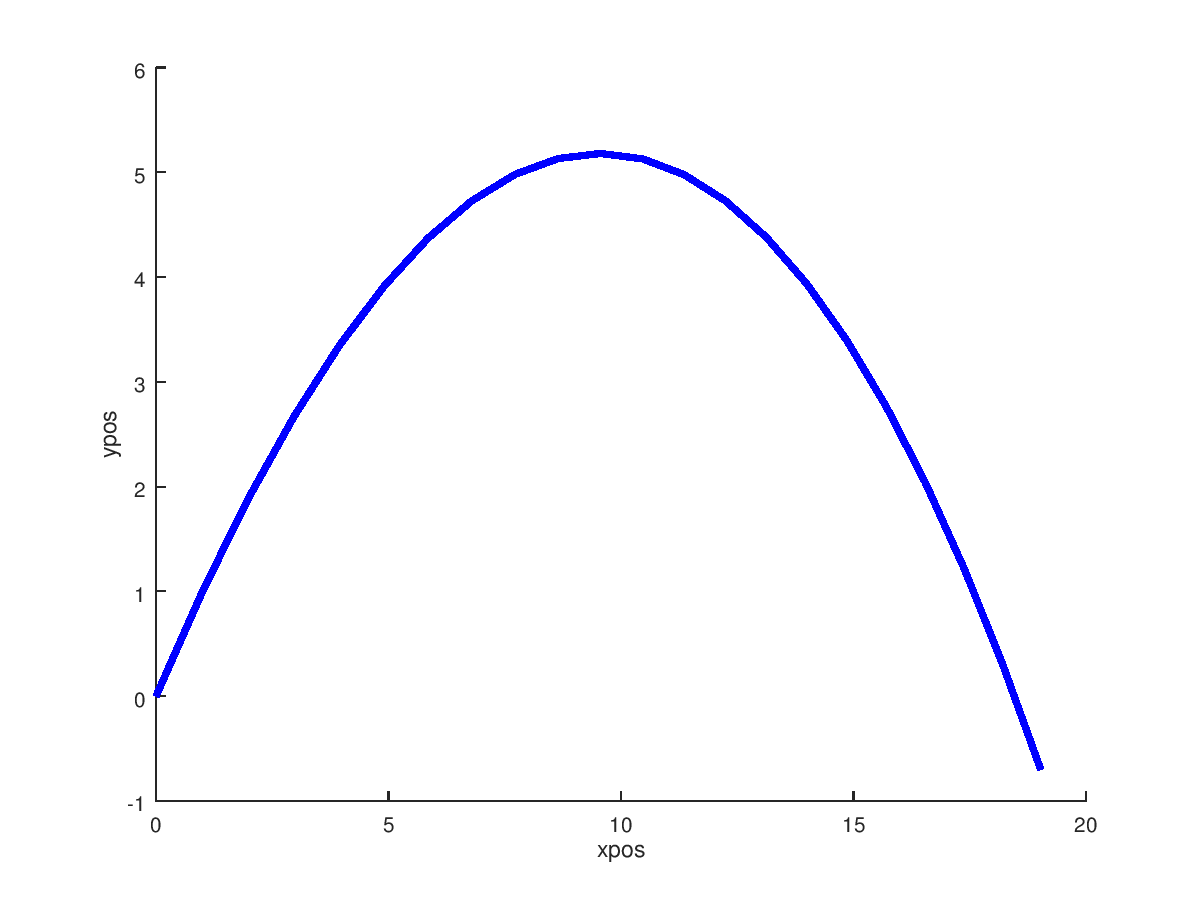
\includegraphics[scale=0.75]{p5}
    {\centering
	    \inputminted[linenos,bgcolor=llgray,frame=lines,framesep=2mm]{octave}{p5.m}}

\end{document}
